%This work is licensed under the Creative Commons License Attribution 4.0 International (CC-BY 4.0)
%https://creativecommons.org/licenses/by/4.0/legalcode
\documentclass[rgb]{standalone}
\usepackage{tkz-euclide}
\definecolor{myorange}{hsb}{0.0833, 1, 0.8}
\definecolor{mygreen}{hsb}{0.3333, 1, 0.8}
\definecolor{myblue}{hsb}{0.5833, 1, 0.8}
\definecolor{mymagenta}{hsb}{0.8333, 1, 0.8}
\begin{document}
	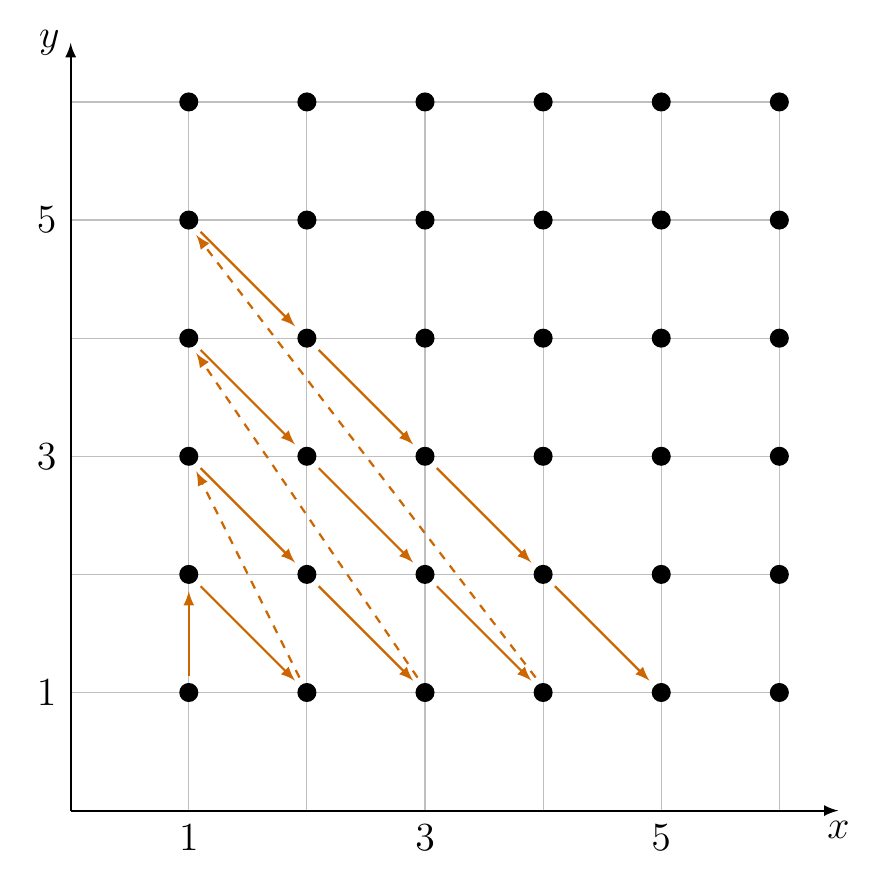
\begin{tikzpicture}[scale=1.5, font=\Large]
		% Coordinate system
		\tkzInit[xmin=0,xmax=6,ymin=0,ymax=6]
		\tkzGrid[color=lightgray]
		\tkzDrawX[thick,label=$x$]
		\tkzDrawY[thick,label=$y$]
		\foreach \i in {1,...,6} {
			\foreach \j in {1,...,6} {
				\node[very thick, draw,circle,fill,inner sep=2] at (\i, \j) {};
			}
		}
		\draw[thick, myorange, -latex] (1,{1+sqrt(2)/10}) -- (1,{2-sqrt(2)/10});
		\foreach \i in {1,...,4} {
			\foreach \j in {1,...,\i} {
				\draw[thick, myorange, -latex] (\j+0.1,1.9+\i-\j) -- (\j+0.9,1.1+\i-\j);
			}
		}
		\foreach \i in {1,...,3} {
			\draw[thick, myorange, dashed, -latex] ({\i+1-sqrt(10)/50},{1+sqrt(10)/25}) -- ({1+sqrt(10)/50},{\i+2-sqrt(10)/25});
		}
		\node[below=0.5mm] at (1,0){$1$};
		\node[below=0.5mm] at (3,0){$3$};
		\node[below=0.5mm] at (5,0){$5$};
		\node[left=0.5mm] at (0,1){$1$};
		\node[left=0.5mm] at (0,3){$3$};
		\node[left=0.5mm] at (0,5){$5$};
	\end{tikzpicture}	
\end{document}